Es stehen ein RLC-Messgerät, ein Oszilloskop und ein Funktionsgenerator zur Ver\-fü\-gung, sowie einige Koaxialkabel und unbekannte Widerstände in einer Box.
\subsubsection*{Direkte Messung der Leitungskonstanten}
Zunächst werden die Leitungskonstanten $R,L,C$ gemessen. Dafür wird ein Koaxialkabel mit einem Widerstand von \SI{50}{\ohm} an den Funktionsgenerator angeschlossen und mit dem RLC-Messgerät werden die Induktivität, der ohmsche Widerstand und die Kapazität des Kabels bei verschiedenen Frequenzen im Bereich von 0.2-\SI{100}{\kilo\hertz} gemessen. Dieser Schritt wird für ein weiteres Koaxialkabel mit \SI{75}{\ohm} wiederholt.
\subsubsection*{Messung der Leitungskonstanten durch Reflexion}
Abbildung \ref{fig:Aufbau} zeigt den Aufbau dieser und der folgenden Messungen.
\begin{figure}[h]
	\centering
	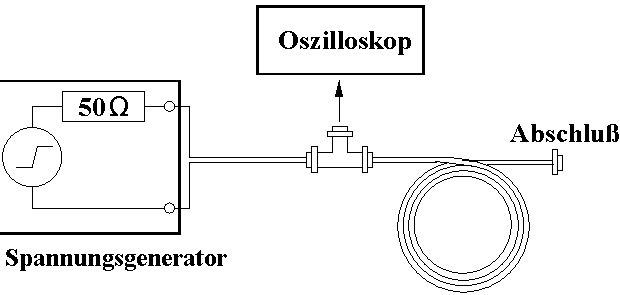
\includegraphics[width=0.7\textwidth]{Aufbau.pdf}
	\caption{Versuchsaufbau \cite{E2}}
	\label{fig:Aufbau}
\end{figure} \\
Um die Leitungskonstanten zu bestimmen werden das Kabel mittlerer Länge am Oszilloskop die Kurven aufgenommen, die entstehen, wenn das Kabel mit offenem und geschlossenem Ende von der anderen Seite mit einem Wechselstrom mit niedriger Frequenz gespeist wird.

\subsubsection*{Messung zur Bestimmung der Dämpfungskonstante}
Um die Dämpfungskonstante bestimmen zu können, wird zuerst ein langes Kabel an den Funktionsgenerator angeschlossen. Am Oszilloskop wird die Fouriertransformierte des Signals angezeigt und ein Bild aufgenommen. Dasselbe wird für ein kurzes Kabel gemacht. Die höheren Moden werden stärker gedämpft als die niedrigen, sodass aus dem Verhältnis der Fourierkoeffizienten der höheren Moden die Dämpfungskonstante bestimmt werden kann.
\subsection*{Abschlusswiderstände}
Der Abschluss des Koaxialkabels wird in drei verschiedene Anschlüsse der Box mit den Widerständen gesteckt und dabei die Signalspannung in Abhängigkeit von der Zeit am Oszilloskop betrachtet. Die aufgenommenen Kurven werden gespeichert. Die Form der Kurven kann dann mit den Kurven in Abbildung \ref{fig:Zeitkonstanten} verglichen werden und so auf den Abschlusswiderstand geschlossen werden.
\subsection*{Mehrfachreflexion}
Durch Reihenschaltung der Kabel mit \SI{50}{\ohm} und \SI{75}{\ohm} kann eine Mehrfachreflexion erzeugt werden. Das Signal am Leitungsende hat dabei die Form wie in \ref{fig:ZeitlicherVerlauf} und wird am Oszilloskop betrachtet. Mit Hilfe der Spannungsdifferenzen zwischen den Plateaus können die Reflexionskoeffizienten bestimmt werden. Aus der Zeit zwischen den Anstiegen können die Längen der Kabel berechnet werden.
